%From: John W Morgan <jmorgan@IAS.EDU>
%Date: Thu, 17 Jul 1997 14:26:01 -0400




\documentclass[10pt]{article}
\usepackage[dvips]{epsfig}
\usepackage{amssymb}




%sample command

%\begin{figure}
%\centerline{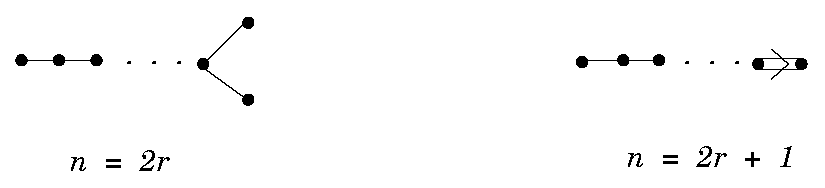
\epsfig{file=fig1.eps}}
%\end{figure}


%variant:

%\centerline{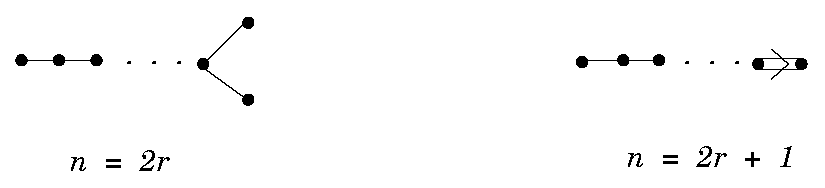
\epsfig{file=fig1.eps,height=3cm}}







%These are the macros which are in common with all of the
% sections in the paper mmr
% Each section, for now, should begin with \documentstyle[11pt,cd]{article}
% and then have \input{mmrmacros} followed by \begin{document}
% The only exception is that the \Label macro is slightly different
% in each file and should be put in separately.
%New CD macros
\newcommand{\cdrl}{\cd\rightleftarrows}
\newcommand{\cdlr}{\cd\leftrightarrows}
\newcommand{\cdr}{\cd\rightarrow}
\newcommand{\cdl}{\cd\leftarrow}
\newcommand{\cdu}{\cd\uparrow}
\newcommand{\cdd}{\cd\downarrow}
\newcommand{\cdud}{\cd\updownarrows}
\newcommand{\cddu}{\cd\downuparrows}
% (S) Proofs.
% (S-1) Head is automatically supplied by \proof.

\def\proof{\vspace{2ex}\noindent{\bf Proof.} }
\def\tproof#1{\vspace{2ex}\noindent{\bf Proof of Theorem #1.} }
\def\pproof#1{\vspace{2ex}\noindent{\bf Proof of Proposition #1.} }
\def\lproof#1{\vspace{2ex}\noindent{\bf Proof of Lemma #1.} }
\def\cproof#1{\vspace{2ex}\noindent{\bf Proof of Corollary #1.} }
\def\clproof#1{\vspace{2ex}\noindent{\bf Proof of Claim #1.} }
% End of Proof Symbol at the end of an equation must precede $$.

\def\endproof{\relax\ifmmode\expandafter\endproofmath\else
  \unskip\nobreak\hfil\penalty50\hskip.75em\hbox{}\nobreak\hfil\bull
  {\parfillskip=0pt \finalhyphendemerits=0 \bigbreak}\fi}
\def\endproofmath$${\eqno\bull$$\bigbreak}
\def\bull{\vbox{\hrule\hbox{\vrule\kern3pt\vbox{\kern6pt}\kern3pt\vrule}\hrule}}
\addtolength{\textwidth}{1in}                  % Margin-setting commands
\addtolength{\oddsidemargin}{-.5in}
\addtolength{\evensidemargin}{.5in}
\addtolength{\textheight}{.5in}
\addtolength{\topmargin}{-.3in}
\addtolength{\marginparwidth}{-.32in}
\renewcommand{\baselinestretch}{1.6}
\def\hu#1#2#3{\hbox{$H^{#1}(#2;{\bf #3})$}}          % #1-Cohomology of #2
\def\hl#1#2#3{\hbox{$H_{#1}(#2;{\bf #3})$}}          % #1-Homology of #2
\def\md#1{\ifmmode{\cal M}_\delta(#1)\else  % moduli space, delta decay of #1
{${\cal M}_\delta(#1)$}\fi}
\def\mb#1{\ifmmode{\cal M}_\delta^0(#1)\else  %moduli space, based, delta
					      %decay of #1
{${\cal M}_\delta^0(#1)$}\fi}
\def\mdc#1#2{\ifmmode{\cal M}_{\delta,#1}(#2)\else    %moduli space, delta
						      %decay, chern class #1
						      %of #2
{${\cal M}_{\delta,#1}(#2)$}\fi}
\def\mbc#1#2{\ifmmode{\cal M}_{\delta,#1}^0(#2)\else   %as before, based
{${\cal M}_{\delta,#1}^0(#2)$}\fi}
\def\mm{\ifmmode{\cal M}\else {${\cal M}$}\fi}
\def\ad{{\rm ad}}
\def\msigma{\ifmmode{\cal M}^\sigma\else {${\cal M}^\sigma$}\fi}
\def\cancel#1#2{\ooalign{$\hfil#1\mkern1mu/\hfil$\crcr$#1#2$}}
\def\dirac{\mathpalette\cancel\partial}
\newtheorem{thm}{Theorem}
\newtheorem{theorem}{Theorem}[subsection]
\newtheorem{proposition}[theorem]{Proposition}
\newtheorem{lemma}[theorem]{Lemma}
\newtheorem{claim}[theorem]{Claim}
\newtheorem{example}[theorem]{Example}
\newtheorem{corollary}[theorem]{Corollary}
\newtheorem{D}[theorem]{Definition}
\newenvironment{defn}{\begin{D} \rm }{\end{D}}
\newtheorem{addendum}[theorem]{Addendum}
\newtheorem{R}[theorem]{Remark}
\newenvironment{remark}{\begin{R}\rm }{\end{R}}
\newcommand{\note}[1]{\marginpar{\scriptsize #1 }} 
\newenvironment{comments}{\smallskip\noindent{\bf Comments:}\begin{enumerate}}{\end{enumerate}\smallskip}

\renewcommand{\thesection}{\Roman{section}}
\def\eqlabel#1{\addtocounter{theorem}{1}
\write1{\string\newlabel{#1}{{\thetheorem}{\thepage}}}
\leqno(\rm\thetheorem)}
\def\cS{{\cal S}}
\def\ov{\overline}













\title{Lecture II-19: $N=2$ Super-symmetric Yang-Mills theories in
dimension four: Part III, Topological Applications}
\author{Edward Witten\thanks{Notes by John Morgan}}
\date{}

\begin{document}
\maketitle


\section{A survey of $N=2$ super-symmetric gauge theories in dimension
four} 

Let us begin with a brief overview of
the range of $N=2$ super-symmetric gauge theories.
We must specify a gauge group $G$ which will be a compact group. 
We shall be doing gauge theory, which means our fields include
a vector multiplet consisting of the gauge fields
and  their super partner fields with values in the adjoint bundle of
the principal $G$-bundle.  We can  also have hypermultiplets.  $N=2$
super-symmetry forces these hypermultiplets to lie in vector bundles
associated to the principal $G$-bundle 
by a representation $\rho\colon G\to Sp(n)$.  This means that the
associated bundles are quaternion bundles.
The most important invariant for the qualitative nature of the theory
is the $\beta$ function, and in particular, the one-loop
$\beta$-function. 
The formula for the one-loop $\beta$-function is
$$\beta_1(g)=\frac{-g^3}{8\pi^2}(4h-c_2(\rho)),$$
where $h$ is the dual coxeter number of the group $G$ and $c_2(\rho)$
is the trace of the quadratic Casimir for $\rho$, normalized so that
the defining representation of $SU(2)$ has $c_2$ equal to one.
Of course, $2h$ is simply $c_2({\rm adjoint})$, the quadratic Casimir of
the adjoint representation of $G$ on its Lie algebra.
There are three possibilites:
\begin{itemize}
\item The one-loop $\beta$-function vanishes.
\item The one-loop $\beta$-function is negative.
\item The one-loop $\beta$-function is positive.
\end{itemize}

Since
$$\tau=\frac{\theta}{2\pi}+\frac{4\pi^2i}{g^2}$$
we have the expansion
$$\mu\frac{d}{d\mu}(\tau)={\rm constant}+\sum_{\ell\ge 1}C\cdot
g^{2\ell}+ \sum c_{n,\ell}g^{2\ell}{\rm exp}(2\pi in \tau),$$
where the constant term is the computed from the one-loop
$\beta$-function,  the higher powers of $g$ arise from higher loop
contributions and the exponential terms come from instanton
corrections (which are of course not seen in perturbation theory).
By super-symmetry $\mu\frac{d}{d\mu}(\tau)$ is a  holomorphic
function, and hence the  positive   powers of $g$ in 
this expansion vanish identically. Thus, if the one-loop $\beta$
function vanishes then $\beta$ vanishes in perturbation theory.
In this case it is believed that $\beta\equiv 0$.  
This result is not completely clear -- it is not always the case in
$N=2$ super-symmetric theories that
the exponentially small terms vanish. (Recall that in the pure
$SU(2)$-theory that we studied last time we found instanton
corrections to $\tau$ which gave exponentially small, but non-zero,
corrections to 
the one-loop $\beta$-function.) On the other hand, one case when the
one-loop $\beta$-function does vanish is when the hypermultiplet
representation $\rho$ is the tensor product of the adjoint
representation of $G$ with the quaternions.  This theory in fact has
$N=4$ super-symmetry. Using this enhanced super-symmetry one can show
that the $\beta$-function vanishes identically. The general belief is
that when the one-loop $\beta$-function vanishes then the
$\beta$-function is identically zero.
When $\beta\equiv 0$, the theory has a well-defined $\tau$ just like
the classical theory. It is believed that in this case there is a
subgroup $\Gamma$ 
of finite index in $SL_2({\bf Z})$  with the
property that the theory 
is invariant under a faithful action of $\Gamma$. Of course, when
$\beta\not= 0$ the theory has a mass scale and $\tau$ is no longer
constant. For these theories one would expect, as we saw for the
$U(1)$-theory in Lecture II-17, that there is not an exact duality
of the theory, but rather that there is an action of the duality group
on the representations of the low energy behaviour of the theory by
Lagrangians. 


When the one-loop $\beta$-function is negative, then the
$\beta$-function is negative, at least for sufficiently high energy
scales.  (The pure $SU(2)$-theory we studied last time is of this
type.) In this case, we have an asymptotically free theory which is a 
good fundamental theory.  That is to say we have a well-defined
{\sl problem} (to describe the low energy effective version of the
theory). We solved this problem in the last 
lecture for $G=SU(2)$ or $SO(3)$ with $\rho$ being the trivial
representation. 

When the one-loop $\beta$-function is positive, we do not have a
well-defined problem, since the theory is not asymptotically
free. Rather these theories are candidate {\sl solutions} to the problems
posed by the theories with one-loop $\beta$-function negative. A
theory $T_{\rm mac}$ with positive $\beta$-functioin
theory is a candidate solution in the sense that its low energy
effective theory is well-defined and infrared free.  It is a solution
to the problem posed by a theory, $T_{\rm mic}$, with negative $\beta$,
if $T_{\rm mic}$ flows in the infrared to $T_{\rm mac}$ in the sense
that at long distances (or equivalently low energies) the correlation
functions of the two theories converge to each other.

The gauge theories we will study today are Lagrangian
models that come by quantizing classical physics.  But there are more 
exotic $N=2$ theories in four-dimensions, some of which come from
string theory. 
Not all of these have Lagrangian formulations.   Whether or not they have
Lagrangians, these $N=2$ supersymmetric  theories
should also lead to four-manifold invariants.  Those without
Lagrangians should lead to four-manifold
invariants which do not have a classical description in terms of the
moduli space of solutions to some differential equation.

\section{From Minkowski space to a compact riemannian
four-manifold} 

Let us fix one of the $N=2$ super-symmetric asymptotically free gauge
theories (one with $\beta<0$). For example, if we wish to study
Donaldson theory we will take pure $N=2$ super-symmetric $SU(2)$-gauge
theory.  But for a while we can be more general.
The theory, as we have discussed it so far, has been on Minkowski
four-space. That is to say, we have written down an action which
involves the integration over Minkowski space of a Lagrangian function
of various fields on this space.
We wish to pass from this to a theory defined on a  compact riemannian
four-manifold.
This passage is carried in two steps -- i) rotating from Minkowski
four-space to 
Euclidean four space, and ii) globalizing to a compact riemannian
four-manifold. 

Let us describe how to  Wick rotate
the theory to Euclidean four-space.  Our theory
consists of  a family of local operators with an operator product
expansion (O.P.E).  A realization of the theory
gives values to the  correlation functions of these operators at
various points of Minkowski four-space.  But there is an open subset
of the complexification of Minkowski four-space where the O.P.E. and the
correlation functions are defined by analytic continuation.  This open
subset contains Euclidean four-space.  In this way we Wick rotate to
define the theory on Euclidean four-space (see, for
example, Kazhdan's lectures from last fall).
In our case we are dealing with (supersymmetric) actions 
$$S=\int_{M^4} {\cal L}$$
which  are integrals of Lagrangians ${\cal L}$ which are analytic
expressions involving fields $\phi$ on the underlying Minkowski space.
These expressions extend to holomorphic expressions on  complexified
Minkowski space and then can be restricted to the Euclidean subspace
to produce a Euclidean Lagrangain ${\cal L}_E$.
The Euclidean action is defined by
$$S_E=\int_{{\bf R}^4}{\cal L}_E.$$
The path integral for a correlation function in Minkowski space is 
$$\int{\cal D}\phi {\cal O}_1(x_1)\cdots{\cal O}_t(x_t)e^{iS},$$
and under this process it Wick rotates to the path integral 
$$\int{\cal D}\phi {\cal O}_1(x_1)\cdots{\cal O}_t(x_t)e^{-S_E}$$
computing the correlation function in Euclidean space.  (Of course,
Feynmann diagram computations of path integrals are easier to do in
the Eulcidean framework and this process is reversed to give answers
in Minkowski space.) For more details on this see the article `Actions
and Reality' by D. Freed.

\subsection{Globalizing by twisting -- the case of the super-symmetric
algebra} 

Now let us examine the question of putting the quantum field theory on
an oriented riemannian four-manifold $X$. Our supersymmetric
theory is defined over four-space by an action $S$ which is an
integral of a Lagrangian function of local fields which are spinors
and vector representations of certain types under $Spin(4)$. Of
course, there are bundles on Minkowski or Euclidean four-space
associated to these representations.
In order to write the `same' action on a  four-manifold $X$
we need to be able to write down the supersymmetric Lagrangian on that
manifold. 
This means that all fields that appear in the Lagrangian
 must be globally defined (as sections of bundles) on $X$.  
This will not in general be the case for the theory as it has been
presented so far because the relevant spin bundles may not exist
globally on $X$.
In fact one sees that the `physically untwisted' theory on a riemannian
four-manifold requires that $X$ be spin and generically breaks all
supersymmetry. 
We have seen before (see Lecture II-??) how to deal
with this problem -- we twist the theory by an appropriate
homomorphism of the spin group $Spin(4)$ to the $R$-symmetry group. 
As we shall see an appropriate twist will both allow us to write down
the Lagrangian on any oriented riemannian four-manifold and also
allow us  to preserve a crucial piece of the supersymmetry.



The decomposition of $\Lambda^2T^*{\bf R}^4$
into self-dual and anti-self-dual components is covered by a decomposition
of the group $Spin(4)$ as $SU(2)_+\times SU(2)_-$.
Fortunately, the $N=2$ the $R$-symmetry group is $U(2)_R=SU(2)_R\times
U(1)_R$.  (The $U(1)_R$ is often absent, e.g., if the hypermultiplet
has nonzero bare  mass. It is also anomalous if $\beta\not= 0$. But
even so, we still have $SU(2)_R$ as an 
$R$-symmetry group.) With this $R$-symmetry group twists  are possible. 
(For $N=1$ the
$R$-symmetry is $U(1)_R$ and there is no possibility for twisting.) 
Recall from the super-homework that the super-symmetric generators are
right-invariant vector fields on ${\bf R}^{4|8}$
$\{Q^i_\alpha\}$ and $\{\overline{Q}_{j\dot\alpha}\}$ where
$1\le i,j,\alpha\le 2$. Both of these sets are acted on
by  $SU(2)_R$ in the standard fashion on the $i,j$ indices.
(The $\alpha$ and $\dot\alpha$ are the spinor indices for
$SU(2)_+\times SU(2)_-$.)  
The actions of the spin group and the $SU(2)_R$ are summarized in the
following table.
$$\begin{array}{|l||c|c|c|}
\hline 
 & \multicolumn{3}{c|} {\rm Transformation\ under} \\
\cline{2-4}
{\rm Charges} &  SU(2)_+ & SU(2)_- & SU(2)_R \\
\hline
 \{Q^i_\alpha\} & \frac{1}{2} & 0 & \frac{1}{2} \\
\hline
\{\overline{Q}_{j\dot\alpha}\} & 0 & \frac{1}{2} &\frac{1}{2} \\
\hline
\end{array}
$$

We define $SU(2)'$ as the diagonal subgroup of
$SU(2)_+\times SU(2)_R$ under the obvious identification of these two groups. 
We shall be interested in the group $SU(2)'\times SU(2)_-$. 
If follows from the information in the table that under $SU(2)'\times
SU(2)_-$ the $\{Q^i_\alpha\}$ 
transform in the representation 
$$(\frac{1}{2}\otimes\frac{1}{2},0)=(0,0)\oplus (1,0).$$
This means that the twisted form of the vector fields $\{Q^i_\alpha\}$
decompose as a complex-valued vector field and a vector field with
values in complex self-dual two-forms.
Similarly, the $\{\overline{Q}_{j\dot\alpha}\}$ transform
in representation 
$$(\frac{1}{2},\frac{1}{2})$$ of this same group and thus are tangent
vectors, so that the  $\{\overline{Q}_{j\dot\alpha}\}$ become vector
fields with values in the complexified tangent bundle. 
Thus, both these representations are vector representations of
$Spin(4)$ and hence
exist globally on any oriented riemannian $4$-manifold.
Also, notice that these representations are naturally real
representations (even though the original ones were only complex).
This means that on the riemannian manifold we can take real fields.

In the superspace language, we are working on the split supermanifold
whose even part is $X$ and whose odd part is the parity reversed
vector bundle
$\wedge^0TX\oplus TX\oplus \wedge ^2_+(TX)$.
On this supermanifold we have a globally defined real vector field 
$Q$ defined as follows.
Suppose that we have  local coordinates $(x^1,\ldots,x^4)$ on an open
subset of $X$. We let $\theta^{\bf R}$ be the natural coordinate in the odd
$\wedge^0TX$-direction and $\theta^i$ be the coordinates in
the odd $TX$-direction determined by the $x^i$. We denote by
$\partial_{{\bf R}^{\rm odd}}$ 
and
$\partial_{i,{\rm odd}}$ be the corresponding vector fields in these
odd directions.  Lastly, $\partial_{i,{\rm even}}$ is the usual
partial derivative in the $x^i$-direction.
We write
$$Q=\partial_{{\bf R}^{\rm odd}}+\theta^i\partial_{i,{\rm even}}.$$
Clearly, as we change local coordinates, this expression is invariant.
This gives us a globally defined real vector field $Q$ on the super
manifold
which is the globalization of the $(0,0)$ component of the twisted
form of the local supersymmetry generators $\{Q_\alpha^i\}$.
It is because of the presence of this one
global, everywhere nonzero, super-symmetric generator satisfying
$Q^2=0$ that we can do global topological quantum field theory on $X$. 




We also have a globally defined one-form $K$ on $X$ with values in vector
fields on the supermanifold derived from the twisted form of
$\{\ov{Q}_{j,\dot\alpha}\}$.  
A formula for it in the same local coordinates is:
$$K=\left(\partial_{i,{\rm odd}}+\theta^{\bf R}\partial_{i,{\rm
even}}\right)dx^i.$$
One sees directly from the formula that $K$ is invariant under  change
of coordinates, and hence is a well-defined global object on $X$. 


It is easy to deduce from the super-Poincar\'e algebra structure, or
from the above explicit formulas,  that
$Q^2=0=\{K,K\}$. 
The direct computation, or the general super-symmetric algebra
structure, also gives
\begin{equation}\label{QK}
\{Q,K\}=d,
\end{equation}
where $d$ is the exterior derivative on $X$.




In fact, by Noether's theorem  there is a local (or unintegrated) form
of these equations.  
Working in Minkowski space and choosing a time-slice $\Gamma$, the
charge $\tilde K$ associated to the operator
$K$ can be written as
$$\tilde K=\int_\Gamma S$$
for a local operator $S$, which is the tensor product of  three-form
on Minkowski space  with a one-form on Minkowski space.
Letting $T$ be the stress-energy tensor (which will exist once we have
managed to formula the theory on a general riemannian manifold) , the
unintegrated form of 
Equation~\ref{QK} is
$$\{Q,S\}=T.$$
This equation can either be viewed as an equation for Poisson bracket
of charges or as an equation for the bracket  of the associated vector
fields (the symplectic gradients of the charges).
Physicists often do not distinguish between the charge and the vector
field. 
In Euclidean space there is the usual relation between the
stress-energy tensor and the translations
\begin{eqnarray*}
P_\mu & = & \int_\Gamma d^3xT_{\mu 0} \\
\ov{Q}_{\dot\alpha} & = & \int_\Gamma d^3xS_{\dot\alpha 0} \\
\{Q^i_\alpha,\ov{Q}_{j\dot\alpha}\} & = &
P_{\alpha\dot\alpha}\delta^i{}_j \\
\{Q_\alpha,S_{\mu\dot\alpha}\} & = & T_{\mu\alpha\dot\alpha}.
\end{eqnarray*}


When we pass from Minkowski space to a riemannian manifold, we can no
longer view $K$ and $Q$ as operators on Hilbert space. Nevertheless,
in this more general context the charges associated to $K$ and 
$Q$ act by Poisson bracket on the local fields to produce new local
fields (or equivalently the associated vector fields act by
differentiation to produce new local fields). 

\subsection{Topological Quantum Field Theory on $X$}

We shall be considering expectation values of products of $Q$-closed
operators. Since the expectation value of any $Q$-exact operator is
trivial (see  Lecture II-??), it follows that the expectation value of any
product of $Q$-closed operators is zero provided that at least one of
them is $Q$-exact.

The fact that $\{Q,T\}=0$ means
that as we vary the metric, the correlation functions change by
the insertion of an operator which is in the image of $Q$.
It then follows that 
the correlation functions we are considering are
independent of the metric.
The operators that we have in mind are the analogues in this more
general gauge theory setting of the Donaldson classes. 
The independence of the metric of the correlation functions of
$Q$-closed operators  is the physics analogue of
the independence of the Donaldson invariants under change of metric.


Let us recall the general scheme of generating operators with values
in higher dimensional differential forms out of local operators with
values in functions.
Here we are generalizing from two-dimensions to four-dimensions the
discussion and results of Lecture II-10.  


Begin with a polynomial function $P$ of degree $d$ on Lie algebra
$\mathfrak{g}$ of the gauge group $G$,
invariant under the adjoint representation. Classically, this produces
a Chern form $P(F_A)$ of degree $2d$ when applied to any connection
$A$ on a principal $G$-bundle. Applying this to the universal
connection on the universal bundle 
over the product of the manifold $X$ with the space ${\cal B}$ of
gauge equivalence classes of configurations yields a closed form of
degree $2d$ on $X\times {\cal B}$. Recall from the last two lectures
that part of the $N=2$ supersymmetric gauge multiplet is an $N=1$
chiral multiplet which includes a scalar field $\phi$ with values in the
adjoint bundle. Quantum mechanically, the
polynomial function $P$ applied to $\phi$ produces a $Q$-closed local
operator ${\cal O}_P^{(0)}$ in the theory.  Applying $K$ repeatedly 
yields operators ${\cal O}_P^{(n)}=K^n{\cal O}_P^{(0)}$.  These are
local operators with values in $n$-forms on $X$. 
For an $n$-cycle $\Sigma^n\subset X$, the operator
$$\int_{\Sigma^n}{\cal O}^{(n)}_P$$
is the analogue of taking the slant product of the Chern form $P(F_A)$
of the universal connection on $X\times {\cal B}$ with the cycle
$\Sigma^n$ to produce a closed form $\mu_P(\Sigma)$ of degree $2d-n$
on ${\cal B}$.  As we shall see, the expectation value
$$\langle \prod_{i=1}^s\int_{\Sigma_i}{\cal O}_P^{(n_i)}\rangle $$
computes 
$$\sum_E\int_{{\cal M}_E}\mu_P(\Sigma_1)\cup\cdots\cup \mu_P(\Sigma_s)$$
where $E$ ranges over the topological types of principal $G$-bundles
over $X$ and where ${\cal M}_E\subset {\cal B}_E$ is the moduli space
of classical solutions.  This integral of course is only taken when
the virtual dimension of ${\cal M}_E$ is equal to
$\sum_{i=1}^s(2d-n_i)$. 


{}From the fact that $\{Q,K\}=d$ and the fact that $\left\{Q,{\cal
O}^{(0)}\right\}=0$,  we have
$$\left\{Q,{\cal O}^{(n)}\right\}=d{\cal O}^{(n-1)}.$$
Thus, we see that the expectation value of
products these operators are topological in nature in the sense
that these expectation values 
depend only on the homology classes of the $\Sigma_i$ in the
four-manifold. 

The $N=2$ supersymmetric  theory that we have been discussing on ${\bf
R}^4$ or Minkowski four-space is induced by dimensionally reducing
from  a theory on ${\bf R}^{6|8}$, i.e., an $N=1$ supersymmetric
theory in six dimensions.  For more details on this, see the
superhomework. 


\subsection{Twisting and globalizing the $N=2$ vector multiplet}

We still have work to do before we have installed the supersymmetric
theories on a riemannian manifold.  So far we have studied the effect
of twisting on the super Euclidean group, and seen how to implement
that on an oriented riemannian manifold.  We must still examine the
fields in the Lagrangian. In this section we study the vector multiplet.


Let us recall the basic configurations of the (untwisted) fields from
an $N=2$ 
vector multiplet in the $N=1$ language. 
First the $N=2$ vector multiplet decomposes as an $N=1$ vector
multiplet 
$${\cal A}=(A,\lambda,D)$$
and an $N=1$ chiral multiplet 
$$\Phi=(\phi,\zeta,F).$$
In the first (vector) multiplet $A$ is a gauge field, $\lambda$ is a spinor
with values in the adjoint bundle and $D$ is a real
auxiliary field with values in the adjoint bundle.
In the chiral multiplet $\phi$ is section of the complexification of
the adjoint bundle, $\zeta$ is a spinor with values in the adjoint
bundle, and $F$ is a complex-valued auxiliary field with values in the
adjoint bundle.
Under the $SU(2)_R$-symmetry the pair $(\lambda,\zeta)$ transform in a
two-dimensional representation denoted $\psi_\alpha^i$ and $\buildrel
\rightarrow\over D = 
(D,{\rm Re}\,F,{\rm Im}\,F)$ transforms under the 
adjoint representation of $SU(2)_R$.

The following table summarizes the $U(1)_R$-charge of the various
fields
$$\begin{array}{|c||c|c|c|c|c|}
\multicolumn{6}{c} {{\rm The} \ N=2\ {\rm Vector\ Multiplet}} \\
\hline
U(1)_R\ {\rm charge} & -2 & -1 & 0 & 1 & 2 \\
\hline
{\rm Field} & \ov{\phi}  &  \ov{\psi}_{\dot\alpha j} & A &
\psi^i_\alpha & \phi \\ 
 & & & \buildrel\rightarrow\over D & & \\
\hline
\end{array}
$$

Now we twist as described above using $SU(2)_R$. The $SU(2)_R$
acts trivially except on $\buildrel\rightarrow\over D$ and on the
fermions, thuys these are the only fields which change character when
we twist.
After twisting the $\psi^i_{\dot\alpha}$ transform in the $(1/2,1/2)$
representation.  This means that after twisting the
$\psi^i_{\dot\alpha}$ become a one-form with values in the adjoint
representation,  denoted $\psi^{(1)}$  on
$X$. Similarly, after 
twisting the $\ov{\psi}_{\alpha j}$ transform in
$(\frac{1}{2}\otimes\frac{1}{2},0)$ and hence decompose as a direct
sum of a function $\psi^{(0)}$ and a self-dual two-form $\psi^{(2)}$. 
The auxiliary field $\buildrel\rightarrow\over D$ also transforms in
$(1,0)$ and hence becomes a self-dual two-form on $X$.

We see that, after
twisting, all these fields exist globally on $X$ since they have
become differential forms. 
This means that as far as pure gauge theories are concerned, we can
write the Lagrangian on any closed oriented $4$-manifold perserving
the supersymmetric charge $Q$.

Let us examine the action of $Q$ on these fields.
The fields $(A,\psi^{(1)},\phi)$ with $Q$, acting as a differential, form a
model of the equivariant cohomology of the gauge group action on the
space of connections.  To make the notation more suggestive of a
differential we let $\delta$ denote the action of $Q$.
Then we have 
\begin{eqnarray*}
\delta A & = & \psi^{(1)} \\
\delta\psi^{(1)} & = & -\dirac_A\phi \\
\delta \phi & = & 0. 
\end{eqnarray*}
The $Q$-closed operators have representatives modulo $Q$-exact
operators using only these fields.
We begin with any operator ${\cal
O}_P^{(0)}=P(\phi)$ given by a 
gauge-invariant polynomial in $\phi$. For example, in the $SU(2)$-case
we take $P(\phi)={\rm Tr}\,\phi^2$. This polynomial has $U(1)_R$-charge four
and corresponds to the Donaldson class $\mu(pt)$ in the fourth
cohomology. From these local operators we build operators with values
in forms ${\cal O}_P^{(j)}=K^j{\cal O}_P^{(0)}$.

The action of $\delta$ on the other fields is:
\begin{eqnarray*}
\delta \ov{\phi} & = & \psi^{(0)} \\
\delta \psi^{(0)} & = & [\phi,\ov{\phi}] \\
\delta\psi^{(2)} & = & F^+_A-\buildrel\rightarrow\over D \\
\delta(F^+_A-\buildrel\rightarrow\over D) & = & [\phi,\psi^{(2)}].
\end{eqnarray*}
Here we are following the notation that the curvature $F_A$ is decomposed
into its self-dual and anti-self-dual components $F^+_A+F^-_A$.



\subsection{Twisting and Globalizing the $N=2$ hypermultiplet} 

Let us turn now to the $N=2$ hypermultiplet. We have
the following table describing the nature of the fields in this $N=2$
multiplet before twisting.

$$\begin{array}{|l||c|c|c|}
\multicolumn{4}{c}{ {\rm The}\ N=2\ {\rm Hypermultiplet}} \\
\hline
{\rm Helicity} & -1/2 & 0 & 1/2 \\
\hline
 U(1)_R-{\rm charge} & -1 & 0 &  1 \\ \hline
 SU(2)_R-{\rm action} & {\rm trivial} & 1/2 & {\rm trivial} \\ \hline
 {\rm Field} & \ov{\lambda}_{\dot\alpha} & M & \lambda_\alpha \\ \hline
 {\rm Type} & -{\rm chirality} & {\rm Boson} & +{\rm chirality} \\
 & {\rm spinor} & & {\rm spinor} \\ \hline
\end{array}
$$
The boson and the spinors of both chiralities in the above table all
take values in the quaternionic bundle over $X$ associated to the
representation $\rho$.

After twisting the boson $M$
becomes a spinor of type $(1/2,0)$, that 
is to say $M$ becomes a plus chirality spinor (a section of the plus
spin bundle). The fermions $\lambda$ and $\ov\lambda$ are unchanged
under twisting since the $SU(2)_R$ acts trivially on them. Thus,
$\lambda$ remains a spinor of plus chirality and $\ov\lambda$ remains
a spinor of minus chirality.
Thus, in order to write the part of the Lagrangian involving the
hypermultiplet we must be able to make sense of the tensor product of
the spin bundles $S^\pm(X)$ of each chirality with the quaternionic
representation $\rho$. (Of course, it is not necessary that the spin
bundles actually exist globally, only that these tensor products exist.)

Assuming that we are in this situation, 
let us describe the action of the differential $Q$ on these fields.
Again denoting it by $\delta$ we get
\begin{eqnarray*}
\delta M & = & \lambda \\
\delta \lambda & = & [a,M] \\
\delta\ov\lambda & = & \dirac(M)+{\rm fermions}.
\end{eqnarray*}





\section{The general form of the high energy computations}

At this point we have succeeded in defining a twisted version of our
$N=2$ super-symmetric gauge theory on any oriented riemannian
four-manifold $X$ for which the bundles $S^\pm(X)\otimes \rho$ are
defined. 
In particular, we have implemented all pure gauge theories  on any
oriented riemannian four-manifold.  
Since the ultraviolet behavior of the theory is independent of the
metric on the manifold and independent of any global topology, we see
that if we began with a fundamental theory (one which has a negative 
$\beta$-function and hence is asymptotically free), then the
implementation of the theory on a complete 
riemannian four-manifold will also be asymptotically free.
Thus, it is a well-defined problem to compute the
correlation functions in this theory.

We are interested in the correlation functions of the
$Q$-closed local operators in the theory.
There is a localization result to the effect that to compute these in
the UV limit one does not need to integrate over the entire infinite
dimensional space of fields, but rather only over the fixed points of
the action of $Q$ on the space of fields (see Lecture II-??).
Another way to think about this is that the correlation functions we
are computing are independent of the metric and we can
compute in the limit when as the metric shrinks to zero, or
equivalently by asymptotic freedom, as the coupling constant goes to
zero.
In the limit we are doing a classical computation over the minima of
the Lagrangian -- this space of minima is exactly the fixed points of
$Q$. 

Let us examine the bosonic part of the fixed point set of $Q$.
{}From the equations above, ignoring the fermion components and working
modulo the action of the gauge group, we see that
the fixed points of $Q$ are given by:
\begin{eqnarray*}
d_A\phi & = & 0  \\
0 & = & F^+_A-\buildrel\rightarrow\over D \label{eqn2} \\
0 & = & \dirac_A(M) 
\end{eqnarray*}
Now using the equations of motion allows us to integrate out the
auxiliary field $\buildrel\rightarrow\over D$ giving the equation
$$\buildrel\rightarrow\over D=\mu(M)$$
where $\mu$ is the hyperk\"ahler moment map.
Thus,  the above system becomes
\begin{eqnarray}
d_A\phi & = & 0  \label{triveqn} \\
F^+_A  & = & \mu(M) \label{SWeqn1} \\
0 & = & \dirac_A(M) \label{diraceqn}
\end{eqnarray}

Away from solutions where $A$ is reducible, the first equation implies
that $\phi=0$, and we can ignore $\phi$ and this equation.  At the
reducible solutions however this equation is important.
Notice that Equations~\ref{SWeqn1} and~\ref{diraceqn} are the
Seiberg-Witten equations in the more general setting where the gauge
group is not required to be $U(1)$. Also, notice that if we are
considering a pure $N=2$ supersymmetric gauge theory (with no
hypermultiplets), then $M=0$ and these equations become the usual
Yang-Mills equations. 


What we see is that our correlation functions will localize to be
integrals over supermanifolds whose underlying geometric manifold is a
disjoint unoin of the moduli spaces
$${\cal M}_E=\left.\cases{ d_A\phi=0 \cr F^+_A=\mu(M) \cr
0=\dirac(M)}\right\}/{\rm (Modulo \ \ gauge)},$$
where the union is taken over all the topological types $E$ for
the principal $G$-bundle. 
 Recall that, assuming that $X$ is compact, there is an index theorem
which computes the virtual dimension of ${\cal M}_E$.  It is
$${\rm virt.\ dim}({\cal
M}_E)=k\left(4h-c_2(\rho)\right)-\frac{1}{2}{\rm
dim}(G)\left(\chi(X)+\sigma(X)\right)-\frac{\sigma(X)}{4}{\rm quaternion\
dim} (\rho),$$
where $k$ is the instanton number of the bundle $E$, $\chi(X)$ is the
Euler characteristic of $X$ and $\sigma(X)$ is its signature.   If
$G$ is simply connected and simple then
$$k=\int_X\frac{{\rm Tr}(F\wedge F)}{8\pi^2}.$$
Notice that if $\beta=0$ then the virtual dimension of ${\cal M}_E$ is
independent of $E$. But when $\beta<0$, the virtual dimension of the
${\cal M}_E$ go to infinity as the instanton number of $E$ goes to
infinity, so that our localization process becomes an integral over an
infinite number of finite dimensional moduli spaces.



As we have said before, we are interested in computing the expectation
values of products of operators  of the form
$$\int_{\Sigma_i}{\cal O}_P^{(k_i)}$$
for an invariant polynomial $P$ on the Lie algebra $\mathfrak{g}$ and for
surfaces $\Sigma_i$ in $X$.
In the case of pure $SU(2)$-gauge theory these operators correspond to
the usual operators in Donaldson theory in the following way. Since
the gauge group is $SU(2)$ the space of irreducible polynomials is
generated by  ${\rm Tr}(\phi^2)=u$. If we use this polynomial
invariant to define ${\cal
O}^{(0)}$, then this operator corresponds to what is usually denoted
$\mu({\rm pt})$ in Donaldson theory.  That is to say, the operator
corresponds to 
the cohomology class on the moduli space which is minus one quarter the
first Pontrjagin class of the $SO(3)$-bundle over the moduli space
given by the based moduli space. Furthermore, the derived operators
$$\int_{\Sigma}{\cal O}^{(k)}$$
correspond to the cohomology classes $\mu([\Sigma])\in H^{4-k}({\cal
M}_E)$. 

One can begin with any 
polynomial function $P$ of degree $d$ on the Lie algebra invariant under
the adjoint 
representation to produce ${\cal O}_P^{(0)}$ and derived  operators of
${\cal O}^{(n)}_P$.  In general, we know from topological considerations
(the K\"unneth formula) how to express the products of integrals of
operators derived out of a decomposable invariant polynomial function
in terms of the integrals of products of operators constructed from
indecomposable invariant functions. Thus, in general it suffices to
work exclusively with products of higher dimensional operators derived
from indecomposable invariant polynomial functions on the Lie algebra.
In the case of $su(2)$
there is only indecomposable invariant polynomial ${\rm Tr}\,\phi^2$.
Hence, it suffices to compute operators derived from this one local
zero dimensional operator. These are the computations we shall do when
we come to Donaldson theory.



In general, to compute a correlation function of the type where ${\cal
O}_P^{(0)}$ 
comes from an invariant polynomial $P$ of degree $d$
$$\langle \prod_{i=1}^s\int_{\Sigma_i}{\cal O}_P^{(b_i)}\rangle$$ 
we must do the integration over all components of the supermanifold of
solutions whose underlying geometric manifold, ${\cal M}_E$, satisfies
$${\rm virt.\ dim}({\cal M}_E)=\sum_{i=1}^s(2d-b_i).$$
Actually, we can do slightly better in the case that $G$ is not simply
connected. We can sum over all principal $G$-bundles $E$
which have a fixed isomorphism class over the two-skeleton of $X$.
(Of course, if $G$ is simply connected, all principal $G$-bundles on
$X$ have isomorphic restriction to the two-skeleton, so in that case
we are summing over all $E$.)



As we have
seen before,  integration of functions over the odd directions in the
supermanifold simply become
integration of differential forms over
the underlying geometric manifold.  The dimension equation ensures
that we are integrating a top dimensional form over the geometric
manifold ${\cal M}_E$ underlying the supermanifold of solutions. 




\subsection{A case when $\beta=0$}


Let us continue with the case when $\beta=0$. 
For simplicity, we take the gauge group $G$ to be a connected
(compact) semi-simple group.
Then, since the ${\cal
M}_E$ all have the same formal dimension, our integration is
over all ${\cal M}_E$ at once.
We have not written down the
Lagrangian explicitly on the curved four-manifold, only on flat
four-space. In putting the theory on a curved space we can add terms
to the action which involve the metric.
Since $\beta=0$, there is a well-defined coupling constant  $\tau$ for
these theories.
  There are two such terms
that preserve the topological invariance, namely:
$$\int_Xf(\tau){\rm Pf}(R)+g(\tau)L(R)$$
where $R$ is the riemann curvature tensor of the metric on the
four-manifold, ${\rm Pf}$ denotes the Pfaffian, and $L$ denotes the
$L$-polynomial, and $f,g$ are holomorphic functions of $\tau$.
(Since $\ov\partial/\partial\ov\tau=\{Q,\cdot\}$, any topological
invariant must be a holomorphic function of $\tau$.)
These give topological terms computing universal multiples of
$\chi(X)$ and $\sigma(X)$, respectively. 
Adding in such terms inserts a multiplicative factor in
the correlation function.
Even if we begin with a classical Lagrangian without these extra
terms, they would be added in the renormalization process, and the
coefficients with which they appear will depend on the explicit nature
of that process.
 Thus, in the end what we are computing is
 of the form
$$q^{a(\tau)\chi(X)+b(\tau)\sigma(X)}\sum_k\langle
\prod_{i=1}^s\int_{\Sigma^{b_i}}{\cal O}^{(b_i)}\rangle_kq^k$$
for functions $a,b$ derived from $f,g$. For example, if $f,g$ are
linear functions of $\tau$, then $a,b$ are constants.
Here, we have fixed the isomorphism class of $E$ over the two skeleton
and indicated by  $k$   the instanton number.
(This action may not be an integer but its value modulo $\bf Z$ is
determined by the isomorphism class of the bundles over the two-skeleton.)
Also, $q=e^{2\pi i\tau}$, and 
the factor $q^k\cdot q^{a(\tau)\chi(X)+b(\tau)\sigma(X)}$ is the value
of the ${\rm exp}(-S)$ on the component  of the moduli space of classical
solutions with instanton number $k$.
Because of the proposed invariance of such a theory under a subgroup
$\Gamma\subset SL_2({\bf Z})$  of finite index, this result should
be a modular form under $\Gamma$ possibly with poles at the cusps of
the quotient of the upper half-plane by $\Gamma$.
We can compute this expression by showing that there is $k_0$ such
that if ${\cal M}_E$ is non-empty then $k\ge k_0$. Also, if $k>>0$
then the index of $\dirac$ is negative and hence generically at least
we expect no solutions to $\dirac(M)=0$ except the trivial solution
$M=0$. Thus, in this range we expect to have to do a computation over
the moduli space ${\cal M}_E^{\rm instantons}$ of solutions to the
anti-self-dual equations.
In this case we are computing
$$\int_{{\cal M}_E^{\rm instanton}}\prod_i\int_{\Sigma_i}{\cal
O}^{(b_i)}\chi({\cal V})$$
where ${\cal V}$ is the obstruction bundle, which in this case is
identified with the cokernel of $\dirac\colon S^+\otimes \rho\to
S_-\otimes \rho$.
One case where we can show that there is a vanishing theorem for
$\dirac$ for all instanton number is the case when the gauge group is
$SU(2)$ and $\rho=su(2)\otimes( {\rm quaternions})$ and the  manifold
is a hyper-K\"ahler manifold. 
 In this case we have $N=4$ supersymmetry, and
${\cal V}$ is identified with the tangent bundle of the instanton
moduli space.
In particular, the virtual dimension of ${\cal M}_E$ is zero.
Thus, in this case, for dimension reaons there can be no positive
dimensional surfaces in the integrals.  That is to say,
we are computing 
$$q^C\sum_kq^k\chi\left({\cal M}_{E_k}\right),$$
for an appropriate constant $C$.
Our conclusion is that this series in $q$ is a modular form (possibly
with poles at infinity), for a subgroup $\Gamma\subset SL_2({\bf Z})$
of finite index. (In fact, $\Gamma$ is the $2$-congruent subgroup
$\Gamma_0^2$.)
This prediction has been compared successfully in some detail to
mathematical computations [Vafa-Witten, {\sl A strong coupling test of
$S$-duality}, Nuclear Physics B, 431 (1994) 3-77].

\subsection{Donaldson Theory}

Now we are ready to specialize to Donaldson theory which is the case
of pure $SU(2)$-theory, pure in the sense that the representaion
$\rho$ is trivial so that there are no hypermultiplets.
As we remarked above the basic operator is ${\cal
O}^{(0)}=u={\rm Tr}\,\phi^2$, coming from the quadratic invariant
polynomial on $su(2)$, and the derived operators ${\cal O}^{(i)},
i=1,\ldots,4$ which 
are to be integrated over $i$-cycles in $X$. 
We denote the various components of the geometric manifold underlying
the supermanifold of classical solutions by ${\cal M}_k$ where
$k\in{\bf Z}$ is the instanton number, i.e., the value of the second
Chern class of the principal $SU(2)$-bundle.
The short distance arguments
above show that
$$\langle \prod_{i=1}^s\int_{\Sigma_i}{\cal
O}^{(b_i)}\rangle_k=\int_{{\cal
M}_k}\mu(\Sigma_1)\cup\cdots\cup \mu(\Sigma_s)$$
where ${\cal M}_k$ is the moduli space of instantons on $X$ with
second Chern class $k$, provided that
$${\rm virt.\ dim}({\cal M}_k)=\sum_{i=1}^s(4-b_i),$$
or equivalently that
$$8k-\frac{3}{2}\left(\chi(M)-\sigma(M)\right)=\sum_{i=1}^s(4-b_i).$$
The integral on the right-hand-side 
is the value of the usual Donaldson polynomial invariant
$$D([\Sigma_1],\ldots,[\Sigma_s])=\int_{{\cal
M}_k}\mu(\Sigma_1^{b_1})\cup\cdots\cup \mu(\Sigma_s^{b_s}).$$  




\section{Low Energy Computations for Donaldson thoery}


{}From now on we concentrate exclusively on Donaldson theory.
To get something interesting we must compare this high energy
computation, which we have just showed limits to the usual Donaldson
polynomial invariants, with a computation using the low energy
effective limit of the theory. In terms of metrics, we imagine a
one-parameter family of metrics $t^2g_0$ for some fixed metric
$g_0$. As we have already remarked, since we are commuting
correlation functions of $Q$-cohomology classes of  operators, the
answers are 
independent of the metric.  As $t\mapsto \infty$ we are recovering the
short distance (or high energy) computations we sketched above and we
find that the results are the Donaldson polynomial invariants.
As $t\mapsto 0$ we can recover the correlation functions by computing
in terms of the space of vacua of the theory.

Thus, we obtain a result of the form
$$\langle\prod_i\int_{\Sigma_i}{\cal O}^{(b_i)}\rangle=\int_{u\
{\rm plane}} E(\Sigma_1,\ldots,\Sigma_s).d\mu$$ 
for an appropriate expression $E$ that depends on the dimensions of the
operators and a measure $d\mu$ on the $u$-plane that depends on the
four-manifold and the path of metrics going to infinity.
(Recall that  all our operators ${\cal O}^{(b_i)}$ are higher
dimensional operators derived from the invariant polynomial ${\rm
Tr}\,\phi^2$.)
It will turn out that as long as $b_2^+(X)>1$, that this integral over
the $u$-plane becomes a sum of two computations, one at each of $u=\pm
1$. When $b_2^+(X)=1$, 
then the answer has three contributions -- discrete contributions at
$u=\pm 1$ as before and an actual integral of a function
over the $u$-plane.
In this case the terms are not topological invariants.
As we vary the metric in a generic one-parameter family
(which of course is all that is necessary to check independence of the
metric) there will be a finite set of points where things degenerate
and on the two sides of each of these points the terms will
have changed.  The changes at $u=\pm 1$ are the wall-crossing formulas
for the Seiberg-Witten invariants whereas the sum of the changes of
the three terms is the wall-crossing formula for the Donaldson
polynomial invariants.



When we do the integral over the $u$-plane, everywhere except at
$u=\pm 1$, we are computing  in a pure $U(1)$-theory, but at $u=\pm 1$ we
cannot ignore the hypermultiplets which become massless at these
points. At $u=\pm 1$ the classical equations are
\begin{eqnarray*}
F_A^+ & = & (M\ov{M})^+ \\
\dirac(M) & = & 0.
\end{eqnarray*}

Here $A$ is a $U(1)$-connection on a line bundle ${\rm det}{S^+\otimes
\cal L}$ and $M$ is 
a section of $S^+\otimes {\cal L}$.
Of course, we must sum over all complex line bundles.
Actually, as we remarked earlier, it is not necessary that $S^+$
exist, only that $S^+\otimes {\cal L}$ exist.  Thus, we are really
summing over $Spin_c$-structures on $X$ (which form a principal
homogeneous set for the group of isomorphism classes of complex line
bundles on $X$).

The appearance of $M$ only at $u=\pm 1$ is of course the reason that
there are delta-function contributions to the measure at these points. 









\subsection{Operators in the effective low energy theory}

In order to do the low energy effective computations we need to know
the image of our operators (defined in the fundamental or high energy
theory) in the low energy effective theory. 
In defining the low energy effective version of
an operator we must integrate out all the high energy modes. This
operation  does not commute with taking products.  Thus, while we
shall see that several of the
elementary operators will correspond in the obvious way, funny things
will happen to products. 
In the high energy theory we have the operator $u={\rm
Tr}\,\phi^2$. We have seen that this operator flows in the low energy
limit to an operator $u$ which we know explicitly.  Its expectation
values are used to parameterize the vacua of the low energy theories. 
Of course, local operators at the point $x$ in the high energy theory
map to local operators at the same point $x$ in the low energy theory,
and hence the 
derivative of a local operator ${\cal O}$ in the high energy theory
maps to derivative of the image $\ov{{\cal O}}$ of ${\cal O}$ in the
low energy theory and similarly $\int_{\Sigma}{\cal O}$ in the high
energy theory flows to $\int_\Sigma\ov{\cal O}$.   
Since the low
energy theory is still $N=2$ supersymmetric, it has the operators $\ov Q$
and  $\ov K$,
which are the images of the operators $Q$ and $K$ in the high energy theory.
Thus,  the image in the low energy theory of $K^nu$ is $\ov K^nu$.
Thus, as long as $\Sigma_1,\Sigma_2$ are disjoint cycles in $X$, the
operation of taking products commutes with integrating over the high
energy modes. This means that 
the high energy operator
$$\int_{\Sigma_1}K^{n_1}u\cdot \int_{\Sigma_2}K^{n_2}u$$
goes in the low energy theory to the product of the images of the
individual operator: 
$$\int_{\Sigma_1}\ov K^{n_1}u\cdot \int_{\Sigma_2}\ov K^{n_2}u$$
as long as
$$\Sigma_1\cap\Sigma_2=\emptyset.$$
Where products will not be preserved in passing to the low energy
effective theory is when the cycles intersect. 
In this case the general form of the answer is that the product
$$\int_{\Sigma_1}K^{n_1}u\cdot \int_{\Sigma_2}K^{n_2}u$$
of high energy operators flows in the low energy limit to  an operator
of the form 
$$\int_{\Sigma_1}\ov K^{n_1}u\cdot
\int_{\Sigma_2}\ov K^{n_2}u+\int_{\Sigma_1\cap\Sigma_2} \ov K^{n_1+n_2}f(u)$$ 
for some function $f(u)$.  
If we take products of more than two operators of this form then there
will be higher corrections
over triple and higher intersections of the cycles.
The reason for all this is that if ${\cal O}_i(x)\mapsto \ov{\cal
O}_i(x)$ then 
$${\cal O}_1(x){\cal O}_2(y)\mapsto \ov{\cal O}_1(x)\ov{\cal
O}_2(y)+\delta(x-y)\tilde {\cal O}_{12}(x)$$
for an appropriate operator $\tilde {\cal O}(x)$ in the low energy
theory. 
In our case if ${\cal O}_i=K^{n_i}u$, then  it must be
the case that $\tilde {\cal O}_{12}=\ov K^{n_1+n_2}f(u)$.
Integrating this result for local operators gives us the formula above
for the image in the low eneryg theory of the product.






Let us simplify the dicussion by supposing that $b_1=0$. Then the only
operators that we need to consider are $u,K^2u,K^4u$.  But there is
never any problem with $K^4u$ since it is a numerical invariant which
is simply the second Chern
class, so that inserting it in a correlation function simply multiples
the expectation value on the bundle by the  second Chern class.
{}From now on we drop this operator from consideration.
Among the remaining operators there are no triple intersections
assuming, as we always can by topological invariance, that the cycles
over which we integrate are in general position.  Furthremore, the only
double intersections are finite sets of points where a pair of
two-cycles meet transversely.  In this case we have that the image of
product of the high energy operators
$$\int_{\Sigma_1}K^{n_1}u\cdot \int_{\Sigma_2}K^{n_2}u$$ 
in the low energy effective theory will be of the form
$$\int_{\Sigma_1}\ov K^{n_1}u\cdot
\int_{\Sigma_2}\ov K^{n_2}u+(\Sigma_1\cap\Sigma_2)T(u),$$ 
where $T$ is a holomorphic  function of $u$ and where
$\Sigma_1\cap\Sigma_2$ denotes the algebraic intersection of
$\Sigma_1$ and $\Sigma_2$.
The reason that $T(u)$ is holomorphic is that since $Q$-closed
operators map to $Q$-closed operators, we must have that the
correction term in formula is $Q$-closed. On the other hand, up to
$Q$-exact terms any $Q$-closed function of $u$ is holomorphic.

\subsection{Warm-up with $U(1)$-theory with a hypermultiplet}

We shall now do a practice computation that will help in learning to
relate the $SU(2)$ and the $U(1)$-theories. 
But we  shall do this practice computation in
a simpler theory -- the $U(1)$-theory with a hypermultiplet and a
minimal Lagrangain, minimal in the sense that we will  omit certain
couplings. 
We simply
take the Lagrangian for the vector multiplet and hypermultiplet as we
wrote them down in flat space with $\tau$ constant. We set $q={\rm
exp}(2\pi i\tau)$. 
The only invariant polynomials for the Lie algebra $u(1)$ are
polynomials in $a$.
 We are 
assuming that $H^1(X)=0$ so that the  operators  under discussion are 
the zero-dimensional operator ${\cal O}^{(0)}=a$ and the
two-dimensional operator ${\cal
O}^{(2)}=c_1({\cal L})$. 
Once again insertion of this latter operator simply multiplies the
correlation function by the first Chern class of the line bundle, and
hence can be ignored.
That is to say the only operators whose expectation values we
need to compute are holomorphic (or polynomial) functions $P(a)$. 

Recall that in this theory the bosonic part of the hypermultiplet
field $M$ becomes after twisting a section of $S^+\otimes {\cal
L}$. This means that ${\cal L}$ should be though of as a
$Spin_c$-structure on $X$ rather than as a complex line bundle.  (We
shall come back to this point in the next lecture.)

Let us suppose that we wish to compute
$\langle P(a)\rangle_\lambda$
for some $Spin_c$-structure $\lambda$.
The high energy arguments outlined above show that this expectation
value concentrates along the geometric manifold ${\cal M}_\lambda$
underlying the moduli space of
solutions to the classical equations for the $Spin_c$-structure
$\lambda$.  Since the value of ${\rm exp}(-S)$ on ${\cal
M}_\lambda$ is $q^{\lambda^2}$, we have:
$$\langle P(a)\rangle_\lambda =q^{\lambda^2}\int_{{\cal M}_\lambda}
P(a).$$ 
Since $a$ is a two-form on ${\cal M}_\lambda$, this integral is equal
to
$$q^{\lambda^2}c_{n_\lambda}\int_{{\cal M}_\lambda}a^{n_\lambda},$$
where $n_\lambda$ is one-half the virtual dimension of ${\cal
M}_\lambda$ and $c_{n_\lambda}$ is the coefficient of $a^{n_\lambda}$
in the Taylor series for $P(a)$ at $a=0$. 
Of course,
$$SW_X(\lambda)=\int_{{\cal M}_\lambda}a^{n_\lambda}$$
is by definition the Seiberg-Witten invariant of the manifold
$X$ evaluated on  the $Spin_c$-structure $\lambda$.
(By convention, all of these integrals are interpreted to be zero if
$n_\lambda$ is not an integer.)
Thus, we have evaluated the expectation value $\langle
P(a)\rangle_\lambda$  to be the coefficient of $a^{n_\lambda}$ in the
Taylor series for $P(a)$ times $q^{\lambda^2}SW_X(\lambda)$.
It is convenient for some of the later computations to rewrite this as 
$$\langle P(a)\rangle_\lambda =q^{\lambda^2}SW_X(\lambda)
\cdot{\rm Res}_{a=0}\left(\frac{da}{a^{1+n_\lambda}}P(a)\right). $$
Summing over all $Spin_c$-structures yields
$$\langle P(a)\rangle =\sum_\lambda\langle P(a)\rangle =
\sum_\lambda q^{\lambda^2}SW_X(\lambda)\cdot {\rm
Res}_{a=0}\left( \frac{da}{a^{1+n_\lambda}}P(a)\right).$$
There is a similar formula when we allow a two-dimensional operator as
well.
\begin{eqnarray*}
\langle P(a)\cdot{\rm exp}\left(\alpha\int_\Sigma{\cal
O}^{(2)}\right)\rangle & = & \sum_\lambda q^{\lambda^ {2}}\cdot
\alpha^{\langle 
c_1(\lambda),\Sigma\rangle} \langle
P(a)\rangle_\lambda \\
&  = & \sum_\lambda q^{\lambda^2}\cdot \alpha^{\langle
c_1(\lambda),\Sigma\rangle}SW_X(\lambda)\cdot{\rm
Res}_{a=0} \left(\frac{da}{a^{1+n_\lambda}}P(a)\right).
\end{eqnarray*}



Now let us generalize this $U(1)$-gauge theory computation by allowing
more general terms that 
preserve topological invariance.
The most general form for the Lagrangian on a
curved manifold $X$, preserving topoloogical invariance, is
$${\cal L}(a,A,M)=\{Q,\cdot\}+\int K^4e(a)+\int g(a){\rm Pf}(R_X)+\int
h(a)L(R_X)$$ 
where $R_X$ is the riemannian curvature tensor of $X$.
By supersymmetry, topological invariance implies that the functions
$e,g,h$ must be holomorphic functions.  Of 
course $\int{\rm Pf}(R_X)$ gives a multiple of the Euler
characteristic whereas $\int L(R_X)$ gives a multiple of
the signature of $X$. 

The expectation value is
$$\sum_\lambda SW(\lambda) {\rm
Res}_{a=0}\left\{\frac{da}{a^{1+n_\lambda}}\left(E(a)^{\lambda^2}
G(a)^{\chi(X)}H(a)^{\sigma(X)}\right)\right\},$$ 
where $G=e^{-g}, H=e^{-h},$ and $E={\rm exp}(-\partial^2e/\partial
a^2)$. 
The reason for the last equation is that since $K(a)=\psi$ and
$K(\psi)=F$, we have
$K(e(a))=e'(a)\psi$ and 
$$K^2(e(a))=e''\psi\wedge \psi+e'(a)K(\psi)=e''\psi\wedge \psi+e'(a)F.$$
Continuing the differentiation, we find that
$$K^4(e(a)=e''(a)F\wedge F+\psi\wedge (\cdots ).$$
In our case all the terms involving $\psi$ vanish since $b_1(X)=0$. 





\subsection{The case of $SU(2)$}

Now we are ready to return to the pure $SU(2)$-theory and understand the
low energy effective computation in terms of the $U(1)$-computations
we just did. Suppose that we fix $\alpha\in {\bf C}$ and a class
$\Sigma\in H^2(X;{\bf C})$.
We wish to compute
$$\langle {\rm exp}\left(\alpha u+\beta\int_{\Sigma}{\cal
O}^{(2)}\right)\rangle_{SU(2)}.$$ 
The general form of the answer will be
$$\langle {\rm exp}(\alpha u+\beta\int_\Sigma{\cal O}^{(2)}\rangle_{u=1}+
\langle {\rm exp}(\alpha u+\beta\int_\Sigma{\cal
O}^{(2)}\rangle_{u=-1}+\int_{u-{\rm plane}}\cdots .$$

Let us see what operators we obtain in the low energy effective
theory.
By our above computations of $K^2(e(a))$ we have
$$\int_\Sigma{\cal O}^{(2)}\mapsto \int_\Sigma K^2u=\int_\Sigma
\frac{\partial u}{\partial a} F+\int_\Sigma\frac{\partial^2 u}{\partial
a^2}\psi\wedge\psi.$$ 
Here, this expression is valid in some region of the $u$-plane and we
have picked one of the possibilities of the $U(1)$-variables  $a$ (remeber
there is an $ISL_2({\bf Z})$-family of such $a$) which is a local
parameter in this region. Near $u=\infty$ we use the usual $a$ but
near $u=1$ we have to use the a different $a$.
If $b_1(X)=0$ then we can drop the second term so that we have
$$\int_\Sigma{\cal O}^{(2)}\mapsto \int_\Sigma
\frac{\partial u}{\partial a} F.$$
Now using the rules for multiplication of the two-dimensional
operators worked out above we see
$${\rm exp}\left(\alpha u+\beta\int_\Sigma{\cal O}^{(2)}\right)\mapsto {\rm
exp}\left(\alpha u+\beta\frac{\partial u}{\partial a} \int_\Sigma
F+\beta^2\Sigma^2T(u)\right).$$ 

Now let us compute the $u=1$ contribution to the Donaldson invariant.
The $a$ we use here is the one produced by the monopole field that is
massless at $u=1$.  We translate this coordinate so that $u=1$
corresponds to $a=0$.
The effective low energy theory is a $U(1)$-theory and is a special
case of the one we discussed in the last section with soem unkonwn
universal functions $e,g,h$ (or equivalently unknown functions $E,G,H$).

So, we have
\begin{eqnarray*} \lefteqn{\langle {\rm exp}\left(\alpha u+\beta\frac{\partial
u}{\partial a}(\Sigma,\lambda)+\beta^2\Sigma^2 T(u)\right)\rangle} \\ 
& = & 2\sum_\lambda SW(\lambda){\rm
Res}_{a=0}\left\{\frac{da}{a^{1+n_\lambda}}{\rm exp}\left(\alpha
u+\beta\frac{\partial 
u}{\partial a}(\Sigma,\lambda)+\beta^2\Sigma^2T(u)\right)
E^{\lambda^2}H^{\sigma(X)}K^{\chi(X)}\right\}. 
\end{eqnarray*}
The factor of $2$ is introduced because of the following reason.
The group of gauge transformations is $SU(2)$-bundle automorphisms,
but its action on the space of connections is not faithful. There is a
central group of order $2$ which acts trivially.  In performing the
path integrals in gauge theory one has to normalize by dividing out by
the volume of the group of gauge transformations. The fact that this
group is twice as big as the group that acts faithfully introduces a
factor of two in the comparison of the path integral with the
topological formulas obtained by integrating over the moduli space.


Of course, by the index theorem, the one-half the dimension of the
moduli space, $n_\lambda$, is a linear function of
$\lambda^2,\chi(X),\sigma(X)$. 

Let us suppose that the manifold $X$ is of simple type (Seiberg-Witten
simple type). By definition this means that all the invariants
$SW_X(\lambda)$ vanish except those for which $n_\lambda=0$. 
Our expression then simplifies to 
$$2\sum_\lambda SW_X(\lambda){\rm Res}_{a=0} \frac{da}{a}{\rm
exp}(\cdots)$$ 
where the unwritten expression is a regular expression in $a$.
We can evaluate at $u=1$ to obtain
$$2\sum_\lambda SW_X(\lambda){\rm
exp}\left(\alpha
u|_{u=1}+(\Sigma,\lambda)\frac{du}{da}|_{u=1}+\Sigma^2T(1)\right) 
\tilde G^{\chi(X)} \tilde H^{\sigma(X)} .$$
Here $\tilde G$ and $\tilde H$ are complex numbers   derived from
$E,G,H$ by setting $u=1$ and using the index theorem (recall
$n_\lambda=0$)  to express $\lambda^2$ as a linear compbination of 
$\chi(X),\sigma(X)$.
To complete determine the answer we must evaluate
$$u(1),
\left.\frac{\partial u}{\partial a}\right|_{u=1}, \tilde G, \tilde H, T(1).$$
Of course, we also have the contribution at $u=-1$ which differs from
this one by the involution $u\mapsto -u$. 


In any event, assuming that, as we shall show in the next lecture,
the integral over 
the $u$-plane does not contribute to the answer when $b_2^+(X)>1$, in
this case the Donaldson polynomial invariant of $X$ is completely
determined by the function $SW_X(\lambda)$ on $Spin_c$ structures and
the explicit determination involves five universal constants that must
be computed.
Fortunately,there is a list of four-manifolds whose Donaldson
invariants are explicitly known, and whose Seiberg-Witten function is
easy to compute, elliptic surfaces.  From these known answers it is an
easy computation to determine the constants.
In fact, there is more than enough information available to determine
these constant since there are infinitely many manifolds for which
both SW and the Donaldson invariants are known.  This gives infinitely
redundant determinations of the constants and gives then infinitely
many checks on the method.  All these computations produce the same
values for the five unknown constants in the above discussion.

The final result is that for manifolds $X$ with $b_2^+(X)>1$ which are
of Seiberg-Witten simple type we have:
\begin{eqnarray*}
\left\langle{\rm exp}\left(\sum_a\beta_a\int_{\Sigma_a}{\cal
O}^{(2)} + \alpha{\cal
O}^{(0)}\right)\right\rangle & = &
2^{1+\frac{1}{4}(7\chi+11\sigma)}\left( {\rm 
exp}\left(\frac{v^2}{2} +2\alpha\right)\sum_\lambda SW_X(\lambda)e^{v\cdot
c_1(\lambda)}\right. \\
& & \left. +i^\Delta{\rm
exp}\left(-\frac{v^2}{2}-2\alpha\right)\sum_\lambda SW_X(\lambda)
e^{-iv\cdot c_1(\lambda)}\right),
\end{eqnarray*} 
where $v=\sum_a\beta_a[\Sigma_a]$ and where
$\Delta=(\chi(X)+\sigma(X))/4$. 
The first of the two terms on the right-hand-side is the contribution
at $u=1$ and the second 
is the contribution at $u=-1$.  It can be derived from the first by
using the involution.

The factor of $2$ in front of the $\alpha$ seems to appear
mysteriously, and is not consistent with the formulas that we
developed because in those formulas the coefficient was always one.
The reason for this descrepancy is that we made an implicit assumption
throughout this 
discussion which now has to be corrected in order to compare with
Donaldson theory. Recall that
in the low energy theory there is a mass scale $\Lambda^2$ and that
the monopoles become massless at $u=\pm \Lambda^2$. We have
implicitly assumed that the monopoles become massless at $u=\pm 1$.
But there is no reason that 
this value of $\Lambda^2$ should be the one that is compatible with
topology. So we should do the computations with an extra unknown
variable $\pm\Lambda^2$ and then determine this variable by comparison
with topological computations in 
examples. Since $\pm\Lambda^2$ is the expectation value of $u$ at the
two special points, the way that $\pm\Lambda^2$ enters the formulas
derived from the low energy computations is as
a multiplicative factor in front of $\alpha$ (the two different signs
appearing in the two different terms). It also changes the
points at which we evaluate the unknown functions, but these values
were not determined directly in terms of $\pm\Lambda^2$, but rather by
comparing with known answers. The fact that $\pm\Lambda^2=\pm 2$ in
order for the field theory computations to give the usual Donaldson
polynomial answers is a reflection of the fact that the simple type 
condition implies that $u^2=4$ in Donaldson theory.
\end{document}



